\documentclass{standalone}
\usepackage[T1]{fontenc}
\usepackage{FiraSans}
\renewcommand{\familydefault}{\sfdefault}

\usepackage{tikz}
\usetikzlibrary{positioning}
\usetikzlibrary{shapes}
\usetikzlibrary{calc}

\begin{document}

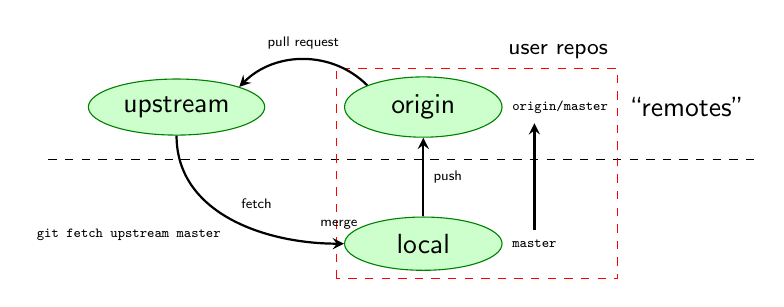
\begin{tikzpicture}
    [repo/.style={ellipse,
		fill=green!20!white,
		draw=green!50!black,
		minimum width=20mm},
    link/.style={-, >=stealth, thick}]

    % remote and local repositories
    \node (upstream) at (0, 0) [repo] {upstream};
    \node (origin) [repo, right=of upstream] {origin};
    \node (local) [repo, below=of origin] {local};

    % repo labels
    \node (origin-master) at (origin.east) [anchor=west] {\tiny \texttt{origin/master}};
    \node (master) at (local.east) [anchor=west] {\tiny \texttt{master}};
    \draw [link, ->] (master) -- (master |- origin-master.south);

    % label of remote repos
    \node (remotes) [right=0mm of origin-master, anchor=west] {``remotes''};

    % separating line between remote and local repos
    \draw [dashed] ($ (upstream.west |- upstream.south) - (5mm, 3mm) $)
	-- ($ (remotes.east |- upstream.south) - (0mm, 3mm) $);

    % box around user's repos
    \draw [dashed, color=red]
	($ (local.west |- local.south) - (1mm, 1mm) $)
	rectangle
	($ (origin-master.east |- origin.north) + (0mm, 1mm) $);
    \node (user-repos) [anchor=south east]
	at ($ (origin-master.east |- origin.north) + (0mm, 1mm) $)
	{\footnotesize user repos};

    % links between repos
    \draw [link, ->] (local) to
	[edge label'={\tiny push}]
	(origin);
    \draw [link, ->] (origin.north west) to
	[out=135, in=45, edge label'={\tiny pull request}]
	(upstream.north east);
    \draw [link, ->] (upstream.south) to
	[out=-90, in=180,
	edge label'={\tiny \texttt{git fetch upstream master}}, edge label={\tiny fetch}]
	(local.west);
    \node at (local.north west) [anchor=east] {\tiny merge};

\end{tikzpicture}
\end{document}
